\documentclass[UTF8]{ctexart}


\usepackage{makecell}
%\usepackage{lipsum}

\usepackage{hyperref}

\usepackage[namelimits]{amsmath} %数学公式
\usepackage{amssymb}             %数学公式
\usepackage{amsfonts}            %数学字体
\usepackage{mathrsfs}            %数学花体


\begin{document}



\author{胡平波\ 党所贵}
%\email{dangsuogui@foxmail.com}
\title{“A”股市场选股模型}

\maketitle
\tableofcontents
\newpage

\section{背景介绍}
\paragraph*{}
近年来,数据分析和AI技术的高速发展将人们带入了大数据时代。在金融领域,尽管人们可得到的数据量越来越多,
但由于知识门槛的限制,普通投资者无法很好的解读上市公司的营业数据和最新的新闻数据。如何有效的利用数据,
特别是文本信息来帮助非专业的普通投资者选股成为当前和今后一段时期内证券公司经纪业务部门亟待解决的问题之一。
本文主要用机器学习算法和图灵机器人来根据普通投资者的实际需求来为用户选择合适的股票。为了帮助用户选股,
本文主要做了以下两个方面的工作:1,对每个公司的投资者成熟度,价格便宜度,交易活跃度和市场关注度分别评级,
将评级结果根据用户的需要传送给用户,并根据评级结果对所有公司进行分类,以便于后续的工作。2,首先,
根据分类结果,在每个类别中,由于财务指标和交易指标都会影响股价,所以以一些经过标准化的财务指标,
交易指标,互联网上的关注度和公众舆情为自变量,15天的收益率为因变量,在这里,财务指标选取主营业务比率,
成本费用利润率,净资产收益率,总资产收益率,投资收益率,每股收益,应收帐款周转率,存货周转率,
总资产周转率,流动比率,利息保障倍数,资产负债率,主营业务现金比率,收益指数,主营业务收入增长率,
净利润增长率,每股权益变化率,市盈率,市净率,交易指标选取当前股价和成交量,前一天股价和成交量,
前两天股价和成交量前5天股价和交易量。具体原因参见 \cite{ph1}。之后,在交叉验证的标准下,用神经网络进行自变量选择和建模。
之后根据当前数据,对公司归类,利用训练好的神经网络对公司做预测,根据预测的收益率大小对公司进行排序,
我们可以认为预测的收益率越大,公司的投资潜力越好,最后把排序结果根据用户的需要传送给用户。

本文分为六部分,第二部分介绍了数据的来源方式以及可得到的数据。第三部分介绍了基本面数据的分析和公司分类,
在这一部分中,可以给用户提供简单的基本面分析结果,同时给所有公司分成了81类,为后续工作做准备。
第四部分介绍了文本信息的处理方法,包括怎么量化上市公司在互联网上的关注度,
怎么利用情感分析将主流媒体和调研报告上的非结构化的文本转化为向量。
第五部分介绍了怎么利用前面所得到的结果建模和预测。第六部分介绍了怎么将我们所得到的结果根据用户需要传递给用户。
\paragraph*{}
本文分为六部分,第二部分介绍了数据的来源方式以及可得到的数据。第三部分介绍了基本面数据的分析和公司分类,
在这一部分中,可以给用户提供简单的基本面分析结果,同时给所有公司分成了81类,为后续工作做准备。
第四部分介绍了文本信息的处理方法,包括怎么量化上市公司在互联网上的关注度,
怎么利用情感分析将主流媒体和调研报告上的非结构化的文本转化为向量。
第五部分介绍了怎么利用前面所得到的结果建模和预测。第六部分介绍了怎么将我们所得到的结果根据用户需要传递给用户。

\section{数据获取}
数据的来源方式以及可得到的数据:
\begin{enumerate}
  \item 通过公开渠道获取A股市场2014年1月1日到2017年7月1日的交易数据,季报,年报和百度搜索指数
  \item 通过网上爬取获取2014年1月1日到2017年7月1日的互联网上主流媒体的相关公司的新闻报道,
  包括新浪财经,第一财经,腾讯财经和凤凰财经。
\end{enumerate}


\section{基本数据分析与公司分类}
\paragraph*{}
在这部分,利用聚类方法,分别根据当前时刻的投资者成熟度,价格便宜度,交易活跃度和市场关注度对A股上市公司分为高,
一般,低三类,这样通过两两组合,A股上市公司就被分为了81类,同一个公司在不同的时刻可能会处于不同的类别中,
这么做的原因是不同的投资成熟度,价格便宜度,交易活跃度和市场关注度的公司特性不一样,不宜放在一起处理。
\paragraph*{}
根据金融学理论,投资者成熟度与流通市值和比例,十大股东持股比例,机构持股比例,股东户数,平均持股数有关。
价格便宜度与每股净资产和盈利,市盈率和市净率,每股现金流,主营收入,主营成本,资产负债率有关。
交易活跃度与创阶段新高/新低,阶段放量/缩量,平台突破,阶段涨幅和换手,阶段振幅有关。
市场关注度与龙虎榜买入净额,机构买入净额,1年内机构买入/持有/卖出评级,机构调研次数有关。
下面以投资者成熟度为例说明如何利用聚类方法将公司分为投资者成熟度高,投资者成熟度一般,
投资者成熟度低这三个等级。其他三种情况类似。根据获得的数据,可以直接算出某个公司在某个时刻的流通市值和比例,
十大股东持股比例,机构持股比例,股东户数,平均持股数。之后利用聚类方法讲这些数据分为三类即把公司在那个时刻分为了三类,
之后在每一类中挑选出一个典型公司的流通市值和比例,十大股东持股比例,机构持股比例,股东户数,平均持股数,
利用金融学知识,即可把这三个典型公司分为高,一般,低三个等级,这样三个类就成功地分为投资者成熟度高,
投资者成熟度一般,投资者成熟度低这三个等级了。
\paragraph*{}
利用公司的当前数据,将聚类的结果放入图灵机器人的知识库,这样可以根据用户的实际需求,给用户提供需要的信息。



\section{非结构文章向量化}
\paragraph*{}
重要媒体或者权威部门发布的相关新闻报道、行业报道等文本类非结构数据,对评价相关企业发展前景、现状有很强的借鉴作用。
使用关键字计频可以将这些文章关联至相关的公司,同时通过自然语言处理的方法,以情感偏向为标准量化文本信息,
转化为结构化的数据,作为后续决策的依据。
\paragraph*{}
我们将文章看成以句子$A_i\ (i=0\cdots n)\ $组成的序列,其长度为$n$,
将其分为$m\ (m \leq n)$组,记为$C_i (i=0 \cdots m-1)$,对于组$C_i (0 \leq i \leq m-1)$计算组中句子的
情感偏向(正面的或者负面的)及概率的均值$\bar{P_i}$,我们将该文章的情感偏向用向量$\boldsymbol{S}$表示,其中
$$
\boldsymbol{S}_i= \begin{cases}
\bar{P_i}, & \mbox{if }C_i\mbox{is positive}\\
-\bar{P_i}, & \mbox{if }C_i\mbox{is negative}\\
0, & \mbox{otherwise}
\end{cases}
$$
使用向量$\boldsymbol{S}$表达文章情感比使用单个标量能够表达更多的信息,使用该向量表达舆论信息,民众评论等非结构
数据对该公司的情感偏向。
\subsection{句子情感偏向}
我们采用机器学习的方法进行句子情感偏向,基本步骤为数据准备、数据预处理、模型建立。
\subsubsection*{数据准备}
\paragraph{获取训练样本集}
使用台湾大学的情感极性词典,其中包含2810个正极性的词语和8276个负极性的词语,具有极高的准确度。可以增加更多金融
点评领域的正极性、负极性的词加入字典以获得更高的准确性。
\paragraph{获取停用词}
句子中往往会有冗余的词语(这样、的等词语),这些词语出现频率高切对语义贡献不大,我们使用中国科学院计算所中文
自然语言处理平台发布的中文停用词表,共有1208个。
\paragraph{验证集}
使用相关的新闻报道作为验证集。
\subsubsection*{数据预处理}
\paragraph{分词}
分词阶段将样本训练集中的句子拆分成词语的组合,使用Jieba进行句子分词处理,处理后的句子由语义单元组成。
\paragraph{去除停用词}
将每个经过分词处理的句子中的停用词删除。
\subsubsection*{训练词向量}
使用Word2Vec的方法将语义单元转化为向量,我们使用gensim将语义单元转化为向量,将每一个句子的每一个语义单元
对应的词向量线性相加,作为该句子的特征表达。以句子特征向量为输入,已知句子情感极性为标签,使用多层感知机(MLP)
进行回归任务学习。
\paragraph{模型验证}
使用验证集中的记录,进行模型验证,评估模型性能。最终我们得到函数$f:C \to S$即每个句子所对应的情感极性及其概率。
\subsection{文章情感偏向向量}
我们使用函数$f$计算组$C_i (i=0 \cdots m-1)$对应的情感极性的均值,获得文章的情感极性表达向量$\boldsymbol{S}$,
在后续的学习任务中,我们使用向量$\boldsymbol{S}$作为该文章的表达。


\section{收益建模与预测}
首先根据分类结果,在每个类别中,将第一部分提到的选取的自变量标准化,并得到相应时间点未来15天内的收益率,得到这些数据后,
在交叉验证的准则下,用神经网络进行自变量选择和不停地优化模型参数,思路如下图:\\
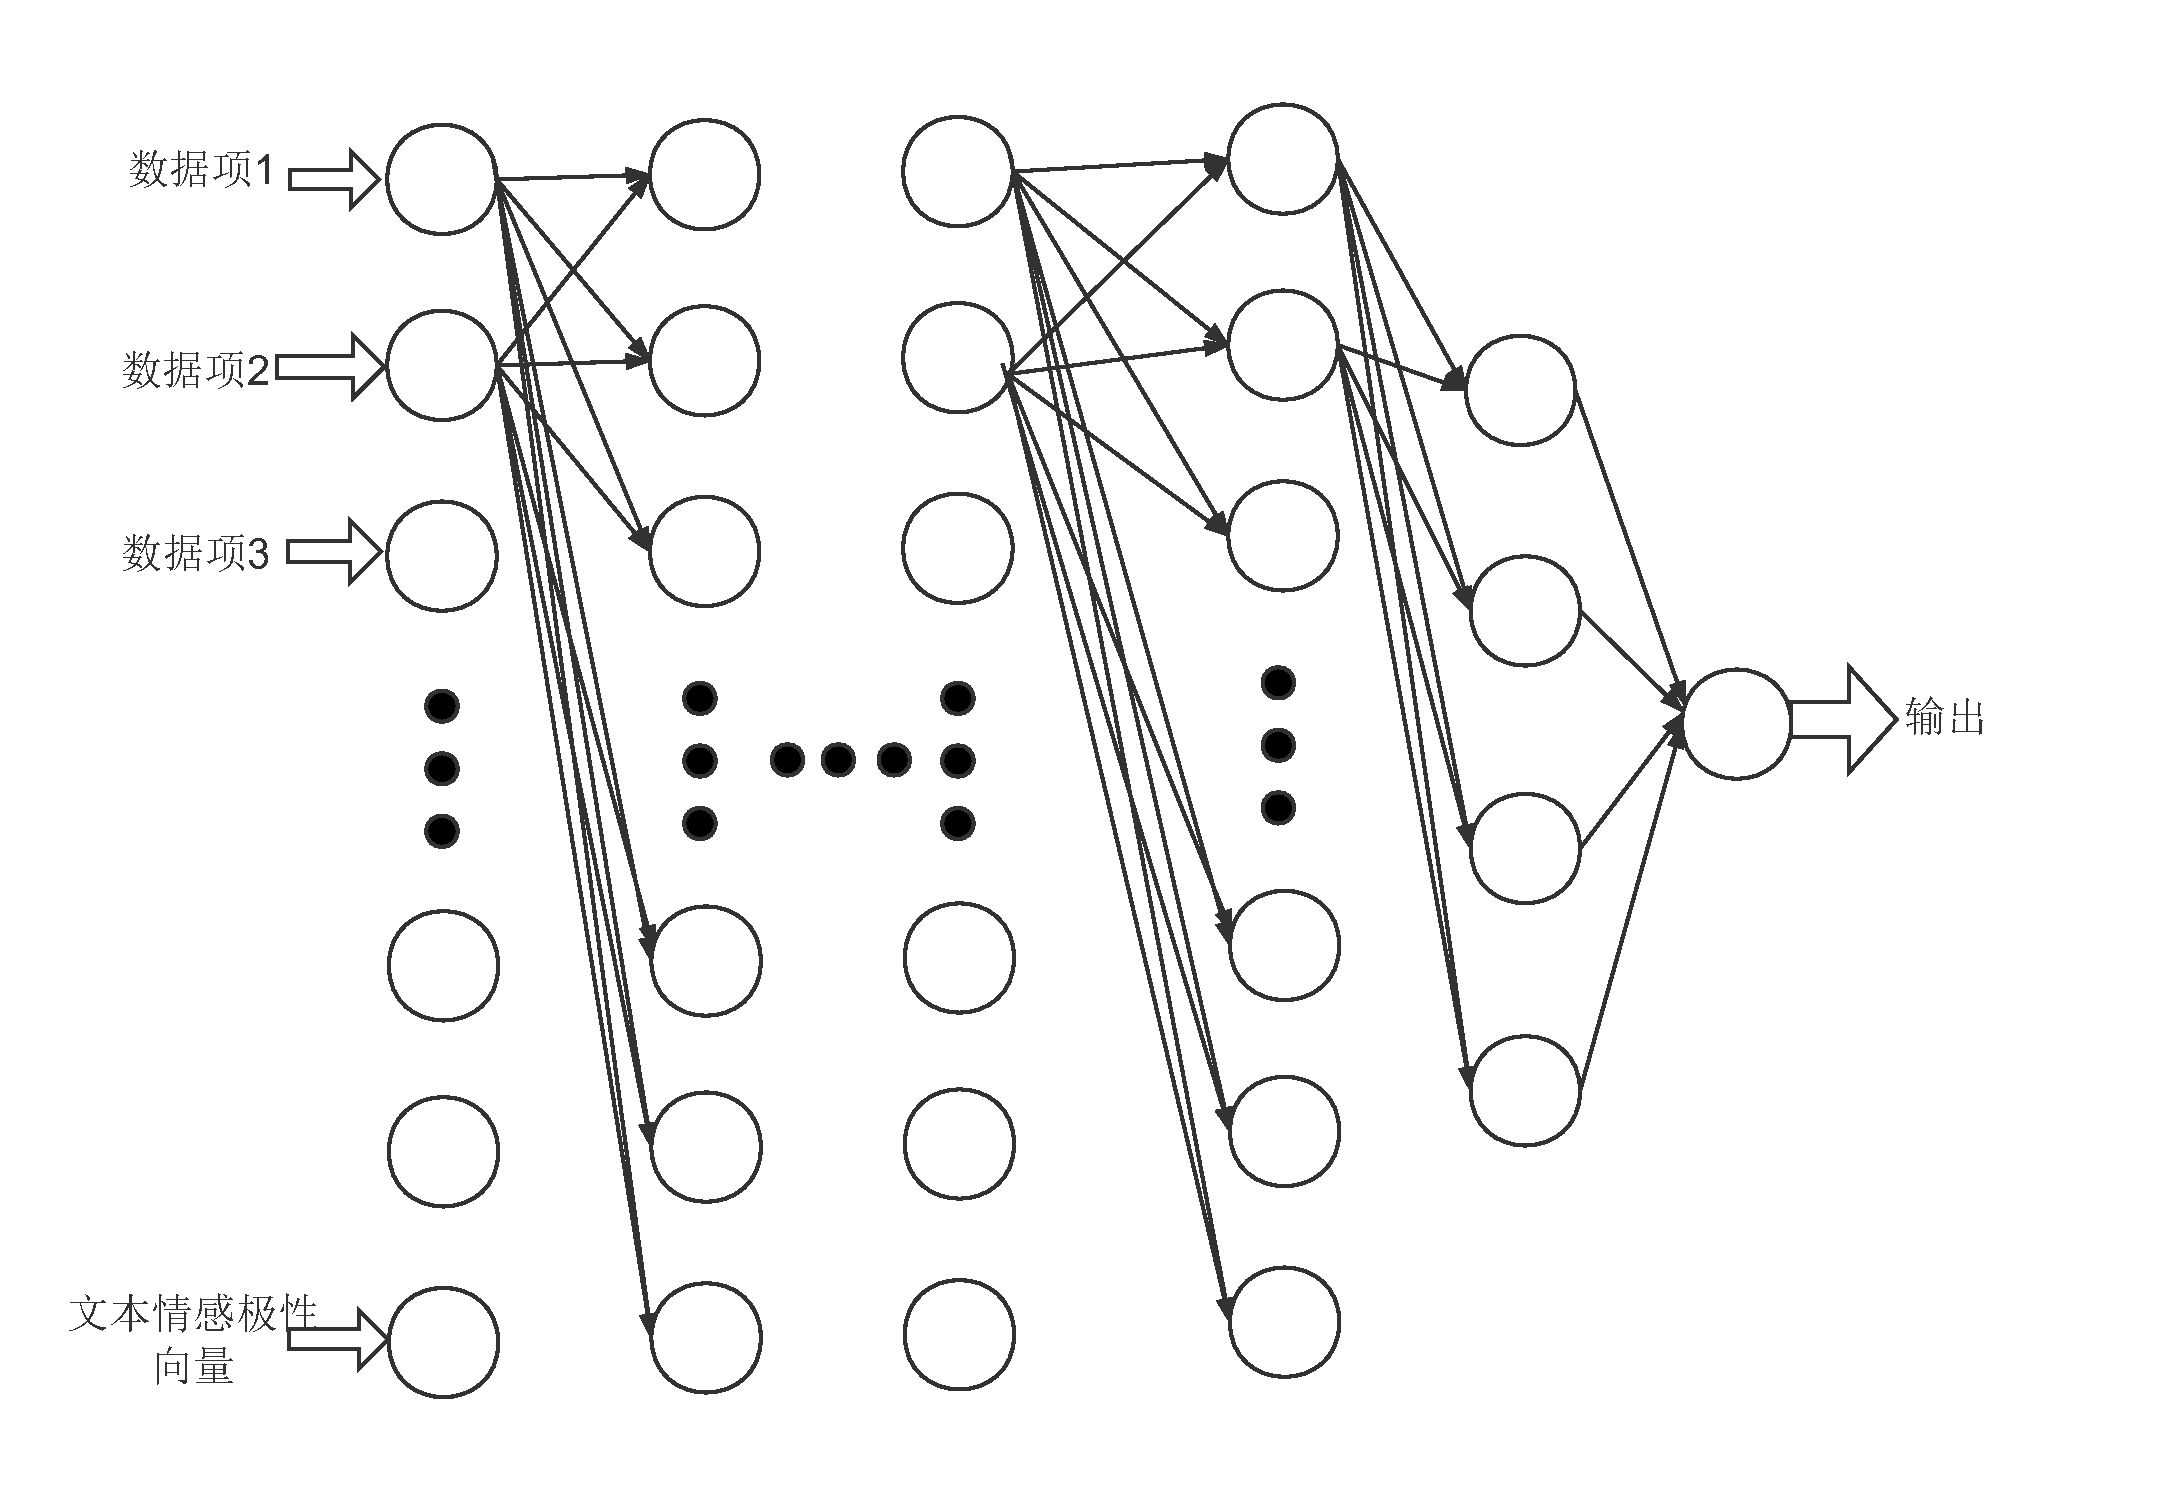
\includegraphics[scale=0.3]{pic1.pdf}
\\然后,在每个类别中,利用训练的模型对公司未来15天的收益率做预测,根据收益率大小对公司进行排序,
这个排序我们可以认为是公司中短期投资潜力的排序,因为公司15天内的收益率越高,这说明投资这个公司中短期越有可能获得高的收益。
最后,把得到的排序结果放入到图灵机器人的知识库中,这样可以根据用户的实际需求,给用户提供需要的信息。
\section{自然语言人机交互}
自然语言人机交互经过多年的发展已经有了很多成熟的解决方案,国内著名的聊天机器人服务提供商图灵机器人,提供自定义聊天机器人的服务。
在我们的项目中,经过建模后,我们的得到公司资者成熟度,价格便宜度,交易活跃度和市场关注度的等级,媒体关注指数,百度搜索指数,媒体评价
情感偏向的数据,将数据添加进图灵聊天机器人知识库,即可通过图灵聊天机器人使用自然语言进行交互。

\bibliographystyle{plain}
\bibliography{cal}
\end{document}
